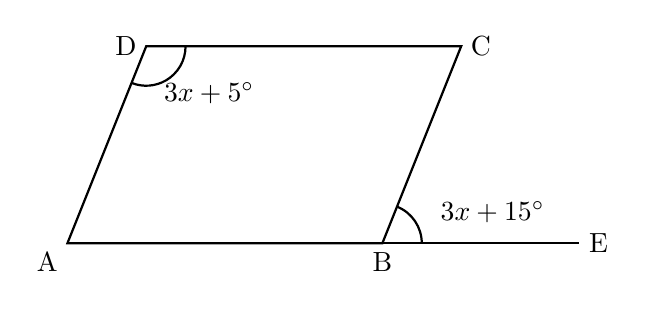
\begin{tikzpicture}[scale=1]

    % Define coordinates for the vertices of the parallelogram
    \coordinate (A) at (0, 0);
    \coordinate (B) at (4, 0);
    \coordinate (C) at (5, 2.5);
    \coordinate (D) at (1, 2.5);

    % Define coordinate for the extended point E on the line AB
    \coordinate (E) at (6.5, 0);

    % Draw the main edges of the parallelogram
    \draw[thick] (A) -- (B) -- (C) -- (D) -- cycle;

    % Draw the extended line from B to E
    \draw[thick] (B) -- (E);

    % Draw the arc for angle ADC (at vertex D)
    % The line DC is horizontal to the right (0 degrees).
    % The line DA goes left and down. Angle is atan2(-2.5, -1) = 248.2 degrees (or -111.8 degrees).
    % The arc is drawn from the DC line to the DA line.
    \draw[thick] (1.5, 2.5) arc (0:-111.8:0.5);
    
    % Add the angle label for ADC inside the parallelogram
    \node at (1.8, 1.9) {$3x+5^{\circ}$};

    % Draw the arc for exterior angle CBE (at vertex B)
    % The line BE is horizontal to the right (0 degrees).
    % The line BC goes right and up. Angle is atan2(2.5, 1) = 68.2 degrees.
    % The arc is drawn from the BE line to the BC line.
    \draw[thick] (4.5, 0) arc (0:68.2:0.5);

    % Add the angle label for CBE
    \node at (5.4, 0.4) {$3x+15^{\circ}$};

    % Add labels to all points exactly as positioned in the image
    \node[below left] at (A) {A};
    \node[below] at (B) {B};
    \node[right] at (C) {C};
    \node[left] at (D) {D};
    \node[right] at (E) {E};

\end{tikzpicture}